%
% test_report_v011.tex
%
% Copyright The TTC 2.0 Contributors.
%
% TTC 2.0 Documentation
%
% This work is licensed under the Creative Commons Attribution-ShareAlike 4.0
% International License. To view a copy of this license,
% visit http://creativecommons.org/licenses/by-sa/4.0/.
%

%
% \brief Test report of the v0.1.1 hardware.
%
% \author Gabriel Mariano Marcelino <gabriel.mm8@gmail.com>
%
% \version 0.2.0
%
% \date 2022/04/22
%

\chapter{Test Report of v0.1.1 Version} \label{anx:test-report-v011}

This appendix is a test report of the first manufactured and assembled PCB (version v0.1.1).

\begin{itemize}
    \item \textbf{PCB manufacturer}: PCBWay (China)
    \item \textbf{PCB assembly}: PCBWay (China)
    \item \textbf{PCB arrival date}: 2022/04/18
    \item \textbf{Execution date}: 2022/04/22 to 2022/04/29
    \item \textbf{Tester}: Gabriel M. Marcelino, Vitória B. Bianchin and Miguel Boing
    \item \textbf{DNP components}: J\_P10, J\_P4, J\_P11, J\_P5, J\_P9, J\_P12, J\_P13, J\_P14, R7, R24, V2, V4, ESD, U12, U13
\end{itemize}

\section{Visual Inspection}

\begin{itemize}
    \item \textbf{Test description/Objective}: Inspection of the board, visually and with a multimeter, searching for fabrication and assembly failures.
    \item \textbf{Material}:
        \begin{itemize}
            \item Multimeter Fluke 17B+
            \item Digital microscope (1000x)
        \end{itemize}
    \item \textbf{Results}: The results of this test can be seen in Figures \ref{fig:ttc2-v011-top} (top view of the board) and \ref{fig:ttc2-v011-bottom} (bottom view of the board).
    \item \textbf{Conclusion}: No problems were identified on this test.
\end{itemize}

\begin{figure}[!ht]
    \begin{center}
        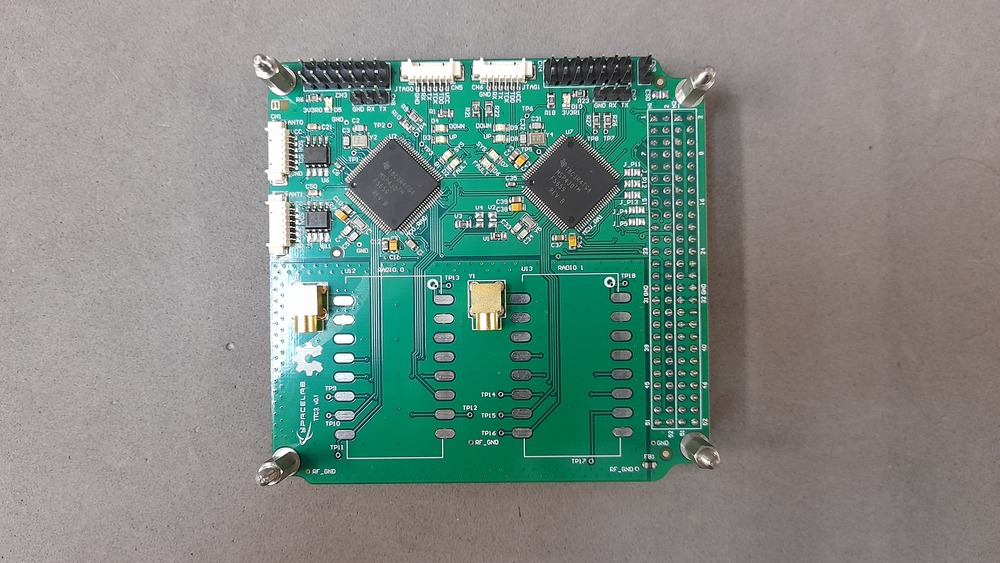
\includegraphics[width=\columnwidth]{figures/v011/ttc2-v011-top.jpg}
        \caption{Top view of the TTC 2.0 v0.1.1 board.}
        \label{fig:ttc2-v011-top}
    \end{center}
\end{figure}

\begin{figure}[!ht]
    \begin{center}
        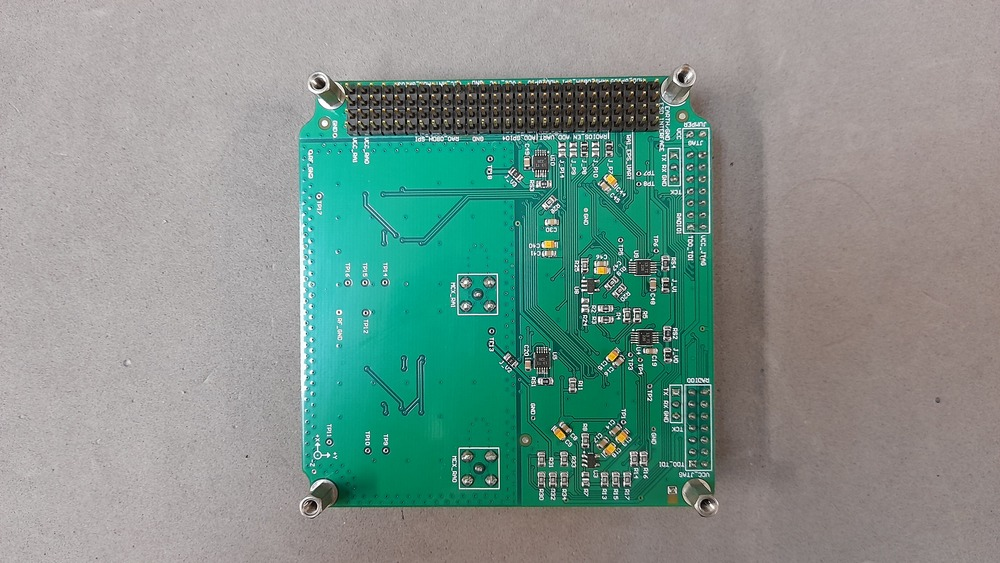
\includegraphics[width=\columnwidth]{figures/v011/ttc2-v011-bottom.jpg}
        \caption{Bottom view of the TTC 2.0 v0.1.1 board.}
        \label{fig:ttc2-v011-bottom}
    \end{center}
\end{figure}

\section{Firmware Programming}

\begin{itemize}
    \item \textbf{Test description/Objective}: Inspection of the board, visually and with a multimeter, searching for fabrication and assembly mistakes.
    \item \textbf{Material}:
        \begin{itemize}
            \item Code Composer Studio v11.2.0
            \item MSP-FET Flash Emulation Tool
            \item USB-UART converter
            \item Screen (Linux software)
        \end{itemize}
    \item \textbf{Results}: %The results of this are available in \autoref{fig:log-first-boot}, where the log messages of the first boot of the board can be seen.
    \item \textbf{Conclusion}: %No problems were identified on this test.
\end{itemize}

%\begin{figure}[!ht]
%    \begin{center}
%        \includegraphics[width=0.7\columnwidth]{figures/v011/log-first-boot.png}
%        \caption{Log messages during the first boot.}
%        \label{fig:log-first-boot}
%    \end{center}
%\end{figure}

\section{Communication Busses}

\begin{itemize}
    \item \textbf{Test description/Objective}: %Test the communication busses of the board, as listed below:
%        \begin{itemize}
%            \item I$^{2}$C Port 0
%            \item I$^{2}$C Port 1
%            \item I$^{2}$C Port 2
%        \end{itemize}
    \item \textbf{Material}:
        \begin{itemize}
            \item Saleae Logic Analyzer (24 MHz, 8 channels)
            \item Saleae Logic software (v1.2.18)
            \item MSP-FET Flash Emulation Tool
        \end{itemize}
    \item \textbf{Results}: %The results of this test can be seen in Figures \ref{fig:test-i2c-0}, \ref{fig:test-i2c-1} and \ref{fig:test-i2c-2}.
    \item \textbf{Conclusion}: %No problems were identified on this test, all buses are working as expected.
\end{itemize}

\section{Sensors}

\subsection{Input Voltage}

\begin{itemize}
    \item \textbf{Test description/Objective}: Verify the input voltage measurements of the board.
    \item \textbf{Material}:
        \begin{itemize}
            \item Code Composer Studio v11
            \item MSP-FET Flash Emulation Tool
            \item USB-UART converter
            \item Screen (Linux software)
        \end{itemize}
    \item \textbf{Results}: .
    \item \textbf{Conclusion:} No problems were identified on this test.
\end{itemize}

\subsection{Input Current}

\begin{itemize}
    \item \textbf{Test description/Objective}: Verify the input current measurements of the board.
    \item \textbf{Material}:
        \begin{itemize}
            \item Code Composer Studio v11
            \item MSP-FET Flash Emulation Tool
            \item USB-UART converter
            \item Screen (Linux software)
        \end{itemize}
    \item \textbf{Results}: .
    \item \textbf{Conclusion:} No problems were identified on this test.
\end{itemize}

\section{Conclusion}

No major problems were identified during the executed tests, all peripherals all working as expected.